\documentclass[18pt,xcolor=table]{beamer}

%!TEX root = ./main.tex
\usepackage {bbm}
\usepackage {textpos}
\usepackage {tikz}
\usepackage {graphicx}


\definecolor{blue1}{RGB}{176,196,222 }
\definecolor{blue2}{RGB}{54,100,139}

\definecolor{grey1}{RGB}{139,139,131}
\definecolor{grey2}{RGB}{235,235,235}

\definecolor{black1}{RGB}{50,50,50}

\mode<presentation>
{
  % \usetheme{Pittsburgh}   
  %\usetheme{Boadilla}  
\usetheme{Madrid}  
  \usefonttheme[onlymath]{serif}
  \setbeamertemplate{items}[circle] 
  \setbeamertemplate{sections/subsections in toc}[circle]
  \setbeamercovered{invisible}
  \setbeamertemplate{navigation symbols}{}
% \usecolortheme{seahorse}
%
%  % Color Theme 
  \setbeamercolor{normal text}{bg=white,fg=black1} %All standard text
  \setbeamercolor{structure}{fg=blue2} %% Table of Contents 

  \setbeamercolor*{frametitle}{fg=black1,bg=grey2} % Frame title colors
%  \setbeamerfont{frametitle}{series=\bfseries}
  \setbeamercolor*{framesubtitle}{fg=blue2} % Frame subtitle color

  \setbeamercolor*{palette primary}{use=structure,fg=black1, bg=grey2} %right bottom
  \setbeamercolor*{palette secondary}{use=structure,bg=blue1} %middle bottom
  \setbeamercolor*{palette tertiary}{use=structure,bg=blue2,fg=grey2} %left bottom

  \setbeamercolor*{block body}{fg=black1,bg=blue1!10} % Color of blocks
  \setbeamercolor*{block title}{parent=structure,fg=black1,bg=blue1} % Block Titles
  \setbeamercolor{alerted text}{fg=blue2!85!black,} % Alerted Text (ie. highlight with \alert)
  \setbeamerfont{alerted text}{series=\bfseries}

  % not sure what these do.
  \setbeamercolor{item projected}{use=item,fg=black1,bg=item.fg!35}
  \setbeamercolor*{block title alerted}{parent=alerted text,bg=black1!15}
  \setbeamercolor*{block title example}{parent=example text,bg=black1!15}
  \setbeamerfont{framesubtitle}{size=\small}
}

\makeatletter
\setbeamertemplate{footline}
{
  \leavevmode%
    \hbox{%
      \begin{beamercolorbox}[wd=.333333\paperwidth,ht=2.25ex,dp=1ex,center]{author in head/foot}%
        \usebeamerfont{author in head/foot}\insertshortauthor%~~\beamer@ifempty{\insertshortinstitute}{}{(\insertshortinstitute)}
      \end{beamercolorbox}%
        \begin{beamercolorbox}[wd=.333333\paperwidth,ht=2.25ex,dp=1ex,center]{title in head/foot}%
        \usebeamerfont{title in head/foot}\insertshorttitle
        \end{beamercolorbox}%
        \begin{beamercolorbox}[wd=.333333\paperwidth,ht=2.25ex,dp=1ex,right]{date in head/foot}%
        \usebeamerfont{date in head/foot}\insertshortdate{}\hspace*{2em}
        \insertframenumber{} / \inserttotalframenumber\hspace*{2ex} 
      \end{beamercolorbox}}%
        \vskip0pt%
}
\makeatother

%\usepackage{kerkis}
\usepackage{helvet} 
\usepackage[T1]{fontenc}
\usepackage[protrusion=true,expansion=true]{microtype}
\usepackage{amsmath}

\renewcommand*{\thefootnote}{\fnsymbol{footnote}}


\pgfdeclareimage[height=1.5cm]{logo}{./logos/hd_logo}
\pgfdeclareimage[height=0.8cm]{small_logo}{./logos/hd_logo}

\AtBeginSection[] { 
  \begin{frame}[plain] 
    \frametitle{\bf Outline:}
    \framesubtitle{~~} 
    \tableofcontents[currentsection] 
  \end{frame} 
  \addtocounter{framenumber}{-1} 
} 

\setbeamercovered{transparent}

%%%%%%%%%%%%%%%%%%%%%%%
% user-defined commands
%%%%%%%%%%%%%%%%%%%%%%%
%!TEX root = ../main.tex


\newcommand{\beq}{\begin{equation}}
\newcommand{\eeq}{\end{equation}}

\newcommand{\eq}[1]{\begin{align*}#1\end{align*}}

\newcommand{\bfi}{\begin{figure}}
\newcommand{\efi}{\end{figure}}

\newcommand{\icg}{\includegraphics}

\newcommand{\bdm}{\begin{displaymath}}
\newcommand{\edm}{\end{displaymath}}

\newcommand{\beqa}{\begin{eqnarray}}
\newcommand{\eeqa}{\end{eqnarray}}

\newcommand{\beqas}{\begin{eqnarray*}}
\newcommand{\eeqas}{\end{eqnarray*}}

\newcommand{\barr}{\begin{array}}
\newcommand{\earr}{\end{array}}

\newcommand{\bit}{\begin{itemize}}
\newcommand{\eit}{\end{itemize}}

\newcommand{\qq}[1]{\qquad \mbox{#1} \qquad}

\def\hyph{-\penalty0\hskip0pt\relax}

% Tikz
\definecolor{blue1}{RGB}{176,196,222 }
\definecolor{blue2}{RGB}{54,100,139}
\definecolor{grey1}{RGB}{139,139,131}
\definecolor{grey2}{RGB}{235,235,235}
\definecolor{black1}{RGB}{50,50,50}


%Spaces
\newcommand{\Sp}[1]{{\cal #1}}
%
\newcommand{\sA}{\Sp{A}}
\newcommand{\sB}{\Sp{B}}
\newcommand{\sC}{\Sp{C}}
\newcommand{\sD}{\Sp{D}}
\newcommand{\sE}{\Sp{E}}
\newcommand{\sF}{\Sp{F}}
\newcommand{\sG}{\Sp{G}}
\newcommand{\sH}{\Sp{H}}
\newcommand{\sI}{\Sp{I}}
\newcommand{\sJ}{\Sp{J}}
\newcommand{\sK}{\Sp{K}}
\newcommand{\sL}{\Sp{L}}
\newcommand{\sM}{\Sp{M}}
\newcommand{\sN}{\Sp{N}}
\newcommand{\sO}{\Sp{O}}
\newcommand{\sP}{\Sp{P}}
\newcommand{\sQ}{\Sp{Q}}
\newcommand{\sR}{\Sp{R}}
\newcommand{\sS}{\Sp{S}}
\newcommand{\sT}{\Sp{T}}
\newcommand{\sU}{\Sp{U}}
\newcommand{\sV}{\Sp{V}}
\newcommand{\sW}{\Sp{W}}
\newcommand{\sX}{\Sp{X}}
\newcommand{\sY}{\Sp{Y}}
\newcommand{\sZ}{\Sp{Z}}

%Vectors
\newcommand{\V}[1]{{\bf #1}}
%
\newcommand{\va}{\V{a}}
\newcommand{\vb}{\V{b}}
\newcommand{\vc}{\V{c}}
\newcommand{\vd}{\V{d}}
\newcommand{\ve}{\V{e}}
\newcommand{\vf}{\V{f}}
\newcommand{\vg}{\V{g}}
\newcommand{\vh}{\V{h}}
\newcommand{\vi}{\V{i}}
\newcommand{\vj}{\V{j}}
\newcommand{\vk}{\V{k}}
\newcommand{\vl}{\V{l}}
\newcommand{\vm}{\V{m}}
\newcommand{\vn}{\V{n}}
\newcommand{\vo}{\V{o}}
\newcommand{\vp}{\V{p}}
\newcommand{\vq}{\V{q}}
\newcommand{\vr}{\V{r}}
\newcommand{\vs}{\V{s}}
\newcommand{\vt}{\V{t}}
\newcommand{\vu}{\V{u}}
\newcommand{\vv}{\V{v}}
\newcommand{\vw}{\V{w}}
\newcommand{\vx}{\V{x}}
\newcommand{\vy}{\V{y}}
\newcommand{\vz}{\V{z}}

\newcommand{\vA}{\V{A}}
\newcommand{\vB}{\V{B}}
\newcommand{\vC}{\V{C}}
\newcommand{\vD}{\V{D}}
\newcommand{\vE}{\V{E}}
\newcommand{\vF}{\V{F}}
\newcommand{\vG}{\V{G}}
\newcommand{\vH}{\V{H}}
\newcommand{\vI}{\V{I}}
\newcommand{\vJ}{\V{J}}
\newcommand{\vK}{\V{K}}
\newcommand{\vL}{\V{L}}
\newcommand{\vM}{\V{M}}
\newcommand{\vN}{\V{N}}
\newcommand{\vO}{\V{O}}
\newcommand{\vP}{\V{P}}
\newcommand{\vQ}{\V{Q}}
\newcommand{\vR}{\V{R}}
\newcommand{\vS}{\V{S}}
\newcommand{\vT}{\V{T}}
\newcommand{\vU}{\V{U}}
\newcommand{\vV}{\V{V}}
\newcommand{\vW}{\V{W}}
\newcommand{\vX}{\V{X}}
\newcommand{\vY}{\V{Y}}
\newcommand{\vZ}{\V{Z}}

\newcommand{\vone}{\V{1}}
\newcommand{\vzero}{\V{0}}
\newcommand{\B}{\V{B}}
\newcommand{\E}{\V{E}}
\newcommand{\Er}{\V{E}_r}
\newcommand{\Es}{\V{E}_s}
\newcommand{\un}{\hat{\vn}}



%Vectors
\newcommand{\T}[1]{\underline{\bf #1}}
%
\newcommand{\ta}{\T{a}}
\newcommand{\tb}{\T{b}}
\newcommand{\tc}{\T{c}}
%\newcommand{\td}{\T{d}}
\newcommand{\te}{\T{e}}
\newcommand{\tf}{\T{f}}
\newcommand{\tg}{\T{g}}
%\newcommand{\th}{\T{h}}
\newcommand{\ti}{\T{i}}
\newcommand{\tj}{\T{j}}
\newcommand{\tk}{\T{k}}
\newcommand{\tl}{\T{l}}
\newcommand{\tm}{\T{m}}
\newcommand{\tn}{\T{n}}
%\newcommand{\to}{\T{o}}
\newcommand{\tp}{\T{p}}
\newcommand{\tq}{\T{q}}
\newcommand{\tr}{\T{r}}
\newcommand{\ts}{\T{s}}
%\newcommand{\tt}{\T{t}}
\newcommand{\tu}{\T{u}}
\newcommand{\tv}{\T{v}}
\newcommand{\tw}{\T{w}}
\newcommand{\tx}{\T{x}}
\newcommand{\ty}{\T{y}}
\newcommand{\tz}{\T{z}}

\newcommand{\tA}{\T{A}}
\newcommand{\tB}{\T{B}}
\newcommand{\tC}{\T{C}}
\newcommand{\tD}{\T{D}}
\newcommand{\tE}{\T{E}}
\newcommand{\tF}{\T{F}}
\newcommand{\tG}{\T{G}}
\newcommand{\tH}{\T{H}}
\newcommand{\tI}{\T{I}}
\newcommand{\tJ}{\T{J}}
\newcommand{\tK}{\T{K}}
\newcommand{\tL}{\T{L}}
\newcommand{\tM}{\T{M}}
\newcommand{\tN}{\T{N}}
\newcommand{\tO}{\T{O}}
\newcommand{\tP}{\T{P}}
\newcommand{\tQ}{\T{Q}}
\newcommand{\tR}{\T{R}}
\newcommand{\tS}{\T{S}}
\newcommand{\tT}{\T{T}}
\newcommand{\tU}{\T{U}}
\newcommand{\tV}{\T{V}}
\newcommand{\tW}{\T{W}}
\newcommand{\tX}{\T{X}}
\newcommand{\tY}{\T{Y}}
\newcommand{\tZ}{\T{Z}}

\newcommand{\tone}{\T{1}}
\newcommand{\tzero}{\T{0}}

%Matrix
\newcommand{\M}[1]{{\mathbb #1}}
%
\newcommand{\mA}{\M{A}}
\newcommand{\mB}{\M{B}}
\newcommand{\mC}{\M{C}}
\newcommand{\mD}{\M{D}}
\newcommand{\mE}{\M{E}}
\newcommand{\mF}{\M{F}}
\newcommand{\mG}{\M{G}}
\newcommand{\mH}{\M{H}}
\newcommand{\mI}{\M{I}}
\newcommand{\mJ}{\M{J}}
\newcommand{\mK}{\M{K}}
\newcommand{\mL}{\M{L}}
\newcommand{\mM}{\M{M}}
\newcommand{\mN}{\M{N}}
\newcommand{\mO}{\M{O}}
\newcommand{\mP}{\M{P}}
\newcommand{\mQ}{\M{Q}}
\newcommand{\mR}{\M{R}}
\newcommand{\mS}{\M{S}}
\newcommand{\mT}{\M{T}}
\newcommand{\mU}{\M{U}}
\newcommand{\mV}{\M{V}}
\newcommand{\mW}{\M{W}}
\newcommand{\mX}{\M{X}}
\newcommand{\mY}{\M{Y}}
\newcommand{\mZ}{\M{Z}}

\newcommand{\mzero}{\M{0}}
\newcommand{\mone}{\M{1}}

% Derivatives
\newcommand{\pd}[2]{\frac{\partial #1}{\partial #2}}
\newcommand{\ppd}[2]{\frac{\partial^2 #1}{\partial #2^2}}
\newcommand{\td}[2]{\frac{\mathrm{d} #1}{\mathrm{d} #2}}

\newcommand{\px}{ \partial_{x} }
\newcommand{\py}{ \partial_{y} }
\newcommand{\pz}{ \partial_{z} }
\newcommand{\pt}{ \partial_{t} }
\newcommand{\ptt}{ \partial_{tt} }

\newcommand{\Div}[1]{\nabla \cdot #1}
\newcommand{\Curl}[1]{\nabla \times #1}
\newcommand{\Ctwo}[1]{\nabla_2 \times #1}
\newcommand{\Grad}[1]{\nabla #1}
\newcommand{\Gperp}[1]{\nabla^\perp #1}
\newcommand{\Lap}[1]{\Delta #1}

%integral d
\newcommand{\dd}[0]{\, \mathrm{d}}

% common discrete quantities
\newcommand{\dt}[0]{\delta t}

% physical variables
\newcommand{\eps}[0]{\epsilon_0}
\newcommand{\mus}[0]{\mu_0}
\newcommand{\boltz}[0]{\kappa_B}
\newcommand{\s}[0]{\alpha}
\newcommand{\vths}[0]{v_{th_\s}}
\newcommand{\vthe}[0]{v_{th_e}}
\newcommand{\vthi}[0]{v_{th_i}}
\newcommand{\Om}[0]{\Omega}
\newcommand{\bdOm}{\partial \Omega}

% bracketing
\newcommand{\inner}[2]{\langle #1, #2 \rangle}
\newcommand{\lb}[0]{\left[}
\newcommand{\rb}[0]{\right]}
\newcommand{\parn}[1]{\left( #1 \right)}
\newcommand{\la}{\langle}
\newcommand{\ra}{\rangle}
\newcommand{\lcb}{\left\{}
\newcommand{\rcb}{\right\}}

\newcommand{\mathAnd}{\,\,\mbox{and}\,\,}
\newcommand{\mathOn}{\,\,\mbox{on}\,\,}

\newcommand{\h}{\hat}
\newcommand{\wh}{\widehat}
%\newcommand{\ul}{\underline}

% math operators
\DeclareMathOperator{\Trace}{trace}
\DeclareMathOperator{\Supp}{supp}
\DeclareMathOperator{\Span}{span}
\DeclareMathOperator{\floor}{floor}
\DeclareMathOperator{\diam}{diam}
\DeclareMathOperator{\ceil}{ceil}
\DeclareMathOperator*{\argmin}{arg\,min}


\newcommand{\red}[1]{\textcolor{red}{#1}}
%added macro definitions here

\usepackage{tikz}
\usepackage{tabularx}
\usetikzlibrary{decorations.markings}
\usetikzlibrary{arrows,positioning} 

\usepackage{cancel}
\usepackage{hyperref}
\usepackage{caption}
\usepackage{subcaption}
\usepackage[]{algorithm}
\usepackage{algpseudocode}
\captionsetup{compatibility=false}


\title[Multigrid]{Introduction to Multigrid Methods}
\subtitle{Day 1: Motivation and Basic Iterative Methods}
\author[Mitchell]{Wayne Mitchell}
\institute{\pgfuseimage{logo}\\Universit\"at Heidelberg\\Institut f\"ur Technische Informatik}
\date[]{\alert{}}


\begin{document}
%!TEX root = ./main.tex
\tikzstyle{block} = [rectangle, draw, rounded corners, shade, top color=white, text width=5em,
  bottom color=blue!50!black!20, draw=blue!40!black!60, very thick, text centered, minimum height=4em]
  \tikzstyle{line} = [draw, -latex']
  \tikzstyle{cloud} = [draw, ellipse,top color=white, bottom color=red!20, node distance=2cm, minimum height=2em]

  \frame{\titlepage}

  \addtobeamertemplate{frametitle}{}{%
      \begin{textblock*}{100mm}(0.9\textwidth,-0.88cm)
    \pgfuseimage{small_logo}
    \end{textblock*}
  }

\AtBeginSection[] { 
  \begin{frame}[t]
    \frametitle{\bf Outline:}
    \framesubtitle{~~} 
    \tableofcontents[currentsection] 
  \end{frame} 
  \addtocounter{framenumber}{-1} 
} 

\let\tempone\itemize
\let\temptwo\enditemize
\renewenvironment{itemize}{\tempone\addtolength{\itemsep}{0.5\baselineskip}}{\temptwo}

\DeclareRobustCommand{\Chi}{\raisebox{2pt}{$\chi$}}
%%%%%%%%%%%%%%%%%%%%%%%%%%%%%%%%%%%%%%%%%%%%%%%%%%%%%%%%%%%%%%%%%%%%%%%%%%%%%%%%

% Slide
\begin{frame}{}
\begin{block}{Day 1 Goals}
\bit
\item Session 1:
\bit
\item Motivations for multigrid
\item Basic iterative methods and convergence theory
\eit
\item Session 2:
\bit
\item Krylov methods and preconditioning
\eit
\item Session 3:
\bit
\item Discussion and hands-on examples
\eit
\eit
\end{block}
\end{frame}

% Slide
\begin{frame}{}
\begin{block}{Resources}
\bit
\item A Multigrid Tutorial. Briggs, Henson, McCormick.
\item Multigrid. Trottenberg, Oosterlee, Sch\"uller.
\item Matrix Computations. Golub, Van Loan.
\eit
\end{block}
\end{frame}

% Slide
\begin{frame}
\frametitle{\bf Outline:}
\framesubtitle{~~}
\tableofcontents
\end{frame}

%%%%%%%%%%%%%%%%%%%%%%%%%%%%%%%%%%%%%%%%%%%%%%%%%%%%%%%%%%%%%%%%%%%%%%%%%%%%%%%%

\section{Introduction and motivation}


% Slide
\begin{frame}{Introduction and motivation}
\begin{block}{Scientific computing}
\bit
\item The three pillars of science: theory, experiments, and \emph{simulation}
\item Computation can allow study of physical phenomena that are difficult, expensive, or infeasible to study with experiments
\item More computational power and more sophisticated algorithms enable more complicated simulations with better accuracy
\eit
\end{block}
\end{frame}

% Slide
\begin{frame}{Introduction and motivation}
\begin{block}{Simulation pipeline}
\bit
\item Physical phenomenon (potential field)
\item Continuous equations (Poisson's equation)
\item Discrete problem formulation (finite difference method)
\item Form discrete system of equations (meshing)
\only<1>{\item Solve the discrete system (linear/non-linear solvers)}
\only<2>{\item \textbf{Solve the discrete system (linear/non-linear solvers)}}
\eit
\end{block}
\end{frame}

% Slide
\begin{frame}{Introduction and motivation}
\begin{block}{Large, sparse linear systems}
\bit
\item Resulting linear systems tend to be large and sparse
\item Size (and conditioning) of the system depends on mesh resolution
\item Solving these linear systems is often a computational bottleneck
\item Want solvers to be:
\bit
\item Efficient (as problem grows, execution time does not suffer)
\item Robust (as conditioning gets worse, convergence does not suffer)
\eit
\eit
\end{block}
\end{frame}

% Slide
\begin{frame}{Introduction and motivation}
\begin{block}{Direct methods}
\bit
\item General purpose direct methods:
\bit
\item Matrix factorizations: Cholesky or LU (Gaussian elimination), QR, SVD 
\item Not generally scalable: $O(N^3)$ computational cost
\eit
\item Problem specific direct methods:
\bit
\item Fast Fourier transform, cyclic reduction, fast multipole, nested dissection, elimination trees
\item More scalabe: $O(N\log N)$ or even $O(N)$ computational cost
\eit
\eit
\end{block}
\end{frame}

% Slide
\begin{frame}{Introduction and motivation}
\begin{block}{Iterative methods}
\bit
\item Basic iterative methods:
\bit
\item Jacobi, Gauss-Seidel
\item Cheap to apply, $O(N)$, but generally poor convergence
\eit
\item Krylov methods:
\bit
\item Conjugate gradient, GMRES, BiCGSTAB
\item Also $O(N)$ with much better convergence, but usually requires preconditioning
\eit
\item Multilevel methods:
\bit
\item $O(N)$ solvers and preconditioners with robust convergence 
\eit
\eit
\end{block}
\end{frame}

% BUT iterative methods don't give you the exact solution, right? Isn't that a problem? No. Tunable accuracy is actually preferred due to discretization accuracy, etc.
% Slide
\begin{frame}{Introduction and motivation}
\begin{block}{Numerical accuracy}
\bit
\item Iterative methods don't give the exact solution ... but ...
\item Typically, we are solving a discrete formulation of the problem
\item Discretization accuracy: the maximum level of accuracy (to the continuous solution) achievable with the given discretization
\item Algebraic accuracy: accuracy of the iterative solution to the true solution of the algebraic problem
\item The goal is to achieve algebraic accuracy on the order of discretization accuracy
\eit
\end{block}
\end{frame}

% Slide
\begin{frame}{Introduction and motivation}
\begin{block}{The importance of complexity}
\bit
\item Larger problems and larger more powerful computers make optimal complexity a necessity!
\eit
\begin{table}
\begin{tabular}{c | c | c | c | c}
$O(N^3)$ alg & $O(N^2)$ alg & $O(N)$ alg & N & Comp speed \\
\hline
0.000001 sec &  0.001 sec & 1 sec & 1 & $10^6$ flops (1980's) \\
1 sec &  1 sec & 1 sec & $10^3$ & $10^9$ flops (1990's) \\
12 days &  17 min & 1 sec & $10^6$ & $10^{12}$ flops (2000's) \\
31,710 years &  12 day & 1 sec & $10^9$ & $10^{15}$ flops (2010's)
\end{tabular}
\end{table}
\end{block}
\tiny{Table credit: Ulrich R\"ude, Erlangen}
\end{frame}


%%%%%%%%%%%%%%%%%%%%%%%%%%%%%%%%%%%%%%%%%%%%%%%%%%%%%%%%%%%%%%%%%%%%%%%%%%%%%%%%

\section{Preliminaries and a model problem}

% Slide 
\begin{frame}{Preliminaries and a model problem}
\begin{block}{Notation}
\bit
\item Matrices: $A$, $P$, $R$
\item Matrix entries: $a_{i,j}$
\item Vectors: $\mathbf{u}$, $\mathbf{f}$, $\mathbf{r}$
\item Vector entries: $u_i$
\item Scalars: $\alpha$, $\gamma$, $\omega$
\item Indices: $i$, $j$, $k$
\eit
\end{block}
\end{frame}

% Slide 
\begin{frame}{Preliminaries and a model problem}
\begin{block}{Definitions}
\bit
\item Inner products: 
\eq{
   \langle \mathbf{x}, \mathbf{y} \rangle = \prod_i x_iy_i
}
\item Vector and matrix norms: 
\eq{
   ||\mathbf{x}|| = \sqrt{\langle \mathbf{x}, \mathbf{x} \rangle} \\
   ||A|| = \sup_{||\mathbf{x}||=1} ||A\mathbf{x}||
}
\item Condition number:
\eq{
   \kappa(A) = ||A^{-1}||\cdot||A|| = \frac{\sigma_{\max}(A)}{\sigma_{\min}(A)} \geq 1
}
\eit
\end{block}
\end{frame}


% Slide
\begin{frame}{Preliminaries and a model problem}
\begin{block}{Model problem: Poisson}
\bit
\item Classic model problem is a simple Poisson problem with zero Dirichlet boundary conditions:
\eq{
\Delta u &= f, & \Omega \\
u &= 0, & \partial \Omega
}
\item Discretizing with finite differences on a regular 1D mesh:
\eit
\eq{
&\frac{-u_{i-1} + 2u_i - u_{i+1}}{h^2} = f_i, & i = 1,2,..., N-1\\
&u_0 = u_N = 0
}
\end{block}
\end{frame}

% Slide
\begin{frame}{Preliminaries and a model problem}
\begin{block}{Model problem: Poisson}
\begin{center}
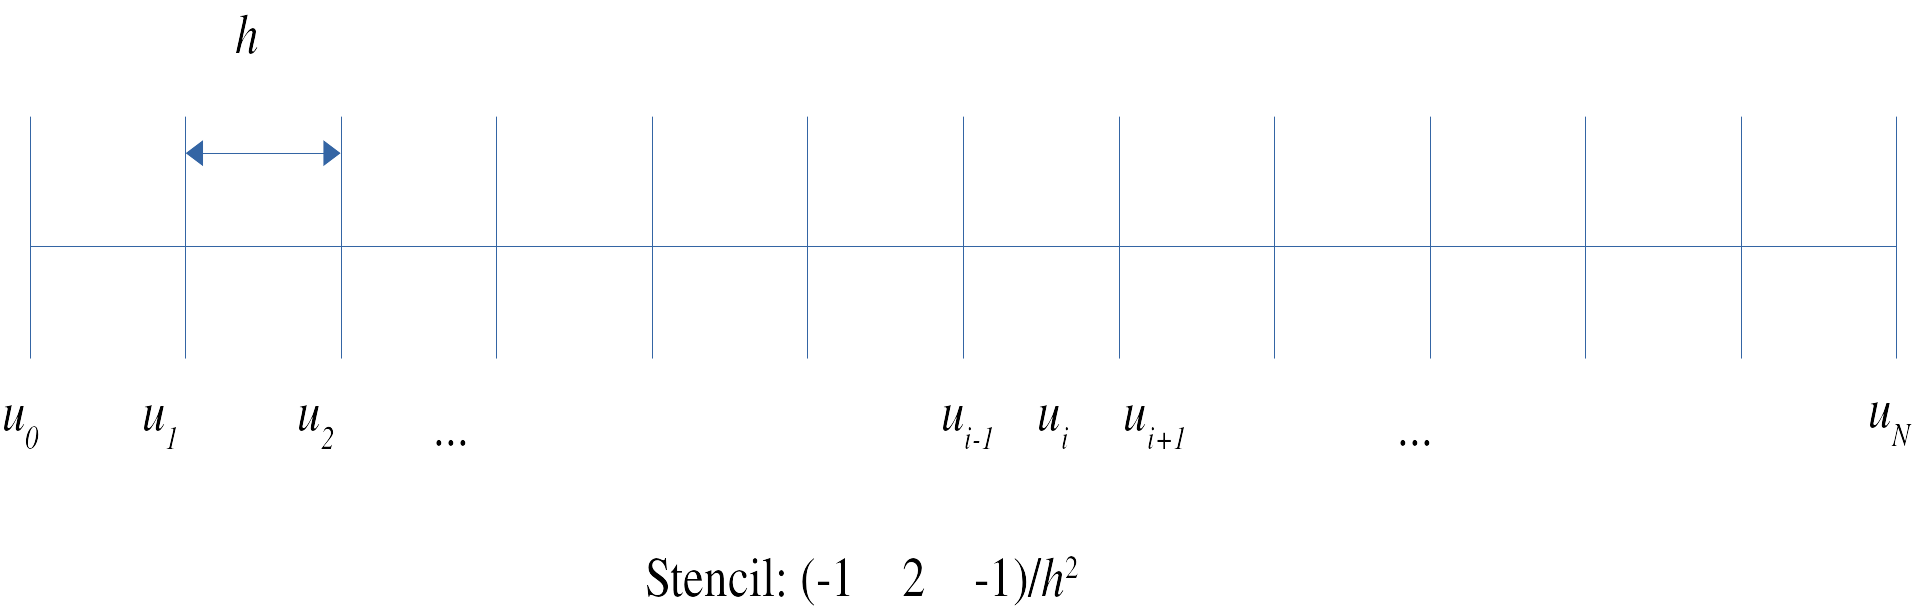
\includegraphics[width=0.7\textwidth]{../figures/1DFDPoisson}
\end{center}
\eq{
\frac{1}{h^2}\begin{bmatrix}
2 & -1 & & & & & & \\
-1 & 2 & -1 & & & & & \\
& -1 & 2 & - 1 & & & & \\
&  & \ddots & \ddots & \ddots & & & \\
& & & & & & & \\
& & & & & -1 & 2 & -1 \\
& & & & & & -1 & 2 \\
\end{bmatrix}
\begin{bmatrix}
u_1 \\
u_2 \\
\\
\vdots \\
\\
\\
u_{N-1} \\
\end{bmatrix}
=
\begin{bmatrix}
f_1 \\
f_2 \\
\\
\vdots \\
\\
\\
f_{N-1} \\
\end{bmatrix}
}
\end{block}
\end{frame}

% Slide 
\begin{frame}{Preliminaries and a model problem}
\begin{block}{Some nice properties}
\bit
\item Sparse
\item Symmetric positive definite (SPD):
\eq{
   A &= A^T \\
   \langle \mathbf{x}, A\mathbf{x} \rangle &> 0 , &\forall \mathbf{x}\neq\mathbf{0}
}
\item Diagonally dominant:
\eq{
   \sum_{j\neq i}|a_{i,j}| \leq |a_{i,i}|, \,\,\forall i
}
\eit
\end{block}
\begin{block}{Less nice properties}
\bit
\item Condition number increases with problem size 
\eit
\end{block}
\end{frame}

%%%%%%%%%%%%%%%%%%%%%%%%%%%%%%%%%%%%%%%%%%%%%%%%%%%%%%%%%%%%%%%%%%%%%%%%%%%%%%%%

\section{Basic iterative methods}

% Slide
\begin{frame}{Basic iterative methods}
\begin{block}{Iterative methods}
\bit
\item Want to solve $A\mathbf{u} = \mathbf{f}$
\item Start with initial guess, $\mathbf{u}^{(0)}$
\item Apply iterative process, $\mathbf{u}^{(i+1)} = S(\mathbf{u}^{(i)})$, $i =0,1,...$
\item Hope that $||\mathbf{u} - \mathbf{u}^{(i)}||$ is acceptably small for reasonable $i$
\eit
\end{block}
\end{frame}


% Slide
\begin{frame}{Basic iterative methods}
\begin{block}{Jacobi iteration}
\bit
\item Simple, point-wise scheme
\item Solve each equation in the system independently, solving the $i^{th}$ equation for the $i^{th}$ unknown
\eit
\eq{
\begin{bmatrix}
a_{0,0} & a_{0,1} & a_{0,2} &... & & & & \\
a_{1,0} & a_{1,1} & a_{1,2} &... & & & & \\
a_{2,0} & a_{2,1} & a_{2,2} & & & & & \\
\ddots&  & \ddots & \ddots & \ddots & & & \\
& & & & & & & \\
& & & & & & & \\
& & & & & & & a_{N-1,N-1} \\
\end{bmatrix}
\begin{bmatrix}
u_0 \\
u_2 \\
\\
\vdots \\
\\
\\
u_{N-1} \\
\end{bmatrix}
=
\begin{bmatrix}
f_0 \\
f_2 \\
\\
\vdots \\
\\
\\
f_{N-1} \\
\end{bmatrix}
}
\end{block}
\end{frame}

% Slide
\begin{frame}{Basic iterative methods}
\begin{block}{Jacobi iteration}
\bit
\item The $i^{th}$ equation is
\eit
\eq{
\sum_j a_{i,j}u_j &= f_i \\
a_{i,i}u_i + \sum_{j\neq i} a_{i,j}u_j &= f_i \\
u_i &= \frac{1}{a_{i,i}} (f_i - \sum_{j\neq i} a_{i,j}u_j)
}
\bit
\item One iteration of Jacobi: for all $i$, set $u^{(k+1)}_i = \frac{1}{a_{i,i}} (f_i - \sum_{j\neq i} a_{i,j}u^{(k)}_j)$
\eit
\end{block}
\end{frame}

% Slide
\begin{frame}{Basic iterative methods}
\begin{block}{Gauss-Seidel}
\bit
\item Gauss-Seidel solves the equations one after another
\item Similar to Jacobi, but uses updated solution
\item One iteration of Jacobi: for $i = 0,1,...$, overwrite $u_i \leftarrow \frac{1}{a_{i,i}} (f_i - \sum_{j\neq i} a_{i,j}u_j)$
\eit
\end{block}
\end{frame}

% Slide
\begin{frame}{Basic iterative methods}
\begin{block}{Matrix representations of iterative methods}
\bit
\item Matrix form of Jacobi:
\eit
\eq{
A\mathbf{u} &= \mathbf{f} \\
(D - L - U)\mathbf{u} &= \mathbf{f} \\
D\mathbf{u} &= \mathbf{f} + (L + U)\mathbf{u} \\
\mathbf{u} &= D^{-1}(\mathbf{f} + (L+U)\mathbf{u})
}
\bit
\item One iteration of Jacobi: $\mathbf{u} \leftarrow D^{-1}(\mathbf{f} + (L+U)\mathbf{u})$
\eit
\end{block}
\end{frame}

% Slide
\begin{frame}{Basic iterative methods}
\begin{block}{Matrix representations of iterative methods}
\bit
\item Matrix form of Gauss-Seidel:
\eit
\eq{
A\mathbf{u} &= \mathbf{f} \\
(D - L - U)\mathbf{u} &= \mathbf{f} \\
(D - L)\mathbf{u} &= \mathbf{f} + U\mathbf{u} \\
\mathbf{u} &= (D-L)^{-1}(\mathbf{f} + U\mathbf{u})
}
\bit
\item One iteration of Gauss-Seidel: $\mathbf{u} \leftarrow (D-L)^{-1}(\mathbf{f} + U\mathbf{u})$
\eit
\end{block}
\end{frame}

% Slide
\begin{frame}{Basic iterative methods}
\begin{block}{General matrix splittings}
\bit
\item Jacobi and Gauss-Seidel are both examples of matrix splittings
\item General matrix splitting: $A = M - N$
\item Iteration: $\mathbf{u} \leftarrow M^{-1}(\mathbf{f} + N\mathbf{u})$
\eit
\end{block}
\end{frame}

% Slide
\begin{frame}{Basic iterative methods}
\begin{block}{Matrix splitting error analysis}
\bit
\item Let $A\mathbf{u} = \mathbf{f}$, $\mathbf{u}^{(k)}$, the $k^{th}$ iterate, and $\mathbf{e}^{(k)} = \mathbf{u}^{(k)} - \mathbf{u}$
\eit
\eq{
M\mathbf{u}^{(k)} &= \mathbf{f} + N\mathbf{u}^{(k-1)} \\
M\mathbf{u} &= \mathbf{f} + N\mathbf{u} \\
\Rightarrow M\mathbf{e}^{(k)} &= N\mathbf{e}^{(k-1)} \\
\mathbf{e}^{(k)} &= M^{-1}N\mathbf{e}^{(k-1)} \\
\mathbf{e}^{(k)} &= (M^{-1}N)^k\mathbf{e}^{(0)}
}
\bit
\item The iteration converges if and only if $(M^{-1}N)^k \rightarrow 0$ as $k\rightarrow \infty$, or equivalently $\rho (M^{-1}N) < 1$
\eit
\end{block}
\end{frame}

% Slide
\begin{frame}{Basic iterative methods}
\begin{block}{Convergence of Jacobi and Gauss-Seidel}
\bit
\item If $A$ is strictly diagonally dominant, then Jacobi converges
\item If $A$ is symmetric positive definite (SPD), then Gauss-Seidel converges
\item Speed of convergence depends on $\rho (M^{-1}N)$ and can be \emph{very} slow
\eit
\end{block}
\end{frame}


%%%%%%%%%%%%%%%%%%%%%%%%%%%%%%%%%%%%%%%%%%%%%%%%%%%%%%%%%%%%%%%%%%%%%%%%%%%%%%%%

\section{Krylov subspace methods}

% Slide
\begin{frame}{Krylov subspace methods}
\begin{block}{Definition of a Krylov subspace}
\bit
\item $\mathcal{K}_r(A,\mathbf{f}) = \text{span}\{\mathbf{f},A\mathbf{f},A^2\mathbf{f},...,A^{r-1}\mathbf{f}\}$
\item Krylov methods minimize an objective over a Krylov subspace
\item Grow the subspace (i.e. increase $r$) on each iteration
\item Subsequent iterates belong to ever richer subspaces and are thus more accurate
\item If $\mathcal{K}_n(A,\mathbf{f}) = \mathcal{R}^n$, minimization yields exact solution
\eit
\end{block}
\end{frame}

% Slide
\begin{frame}{Krylov subspace methods}
\begin{block}{Gradient descent}
\bit
\item Assume $A$ is SPD
\item Recast $A\mathbf{u} = \mathbf{f}$ as a minimization problem:
\eq{
   \phi(\mathbf{u}) = \frac{1}{2}\mathbf{u}^TA\mathbf{u} - \mathbf{u}^T\mathbf{f}
}
\item Note that $-\nabla \phi(\mathbf{u}) = \mathbf{f} - A\mathbf{u}$
\item Thus $\phi(\mathbf{u})$ is minimized at the solution $A^{-1}\mathbf{f}$ and the direction of \emph{steepest descent} towards that minimum is in the direction of the residual, $\mathbf{r} = \mathbf{f} = A\mathbf{u}$
\eit
\end{block}
\end{frame}

% Slide
\begin{frame}{Krylov subspace methods}
\begin{block}{Gradient descent}
\bit
\item $A$ is SPD means we can define the $A$-norm:
\eq{
   ||\mathbf{u}||^2_A = \langle \mathbf{u}, A\mathbf{u} \rangle = \mathbf{u}^TA\mathbf{u}
}
\item If $A\mathbf{\tilde{u}} = \mathbf{f}$ and $\mathbf{u}$ is an approximate solution iterate, then 
\eq{
   ||\mathbf{u} - \mathbf{\tilde{u}}||^2_A = \mathbf{u}^TA\mathbf{u} - 2\mathbf{u}^T\mathbf{f} + ||\mathbf{\tilde{u}}||_A
}
\item Thus, minimizing $\phi(\mathbf{u})$ means minimizing the $A$-norm of the error along a given search direction
\eit
\end{block}
\end{frame}

% Slide
\begin{frame}{Krylov subspace methods}
\begin{block}{Gradient descent}
\bit
\item $\mathbf{r}$ definest the search direction, and $\alpha = \langle \mathbf{r}, \mathbf{r} \rangle / \langle \mathbf{r}, A\mathbf{r} \rangle$
\item $\alpha$ is chosen by an exact line search to minimize $\phi(\mathbf{u} + \alpha \mathbf{r})$
\eit
\end{block}
\begin{algorithm}[H]
\caption{Gradient descent}
\begin{algorithmic}
\State Set $\mathbf{u}$ initial guess
\For{k = 0,1,...}
\State $\mathbf{r} \leftarrow \mathbf{f} - A\mathbf{u}$
\State $\alpha \leftarrow \langle \mathbf{r}, \mathbf{r} \rangle / \langle \mathbf{r}, A\mathbf{r} \rangle$
\State $\mathbf{u} \leftarrow \mathbf{u} + \alpha\mathbf{r}$
\EndFor
\end{algorithmic}
\end{algorithm}
\end{frame}

% Slide
\begin{frame}{Krylov subspace methods}
\begin{block}{Gradient descent}
\bit
\item Again, convergence can be prohibitively slow if $\kappa(A)$ is large
\item Level curves of objective function, $\phi$, are elongated
\item Minimization looks like finding the lowest point in a relatively flat, steep-sided valley
\eit
\end{block}
\end{frame}

% Slide
\begin{frame}{Krylov subspace methods}
\begin{block}{Conjugate Gradient}
\bit
\item Grandient descent can be improved by orthogonalizing search directions
\item Rather than using the residual (direction of steepest descent), orthogonalize the residual against previous search directions
\item Search directions, $\mathbf{p}_k$, are $A$-orthogonal to eachother: $\mathbf{p}_k\in\text{span}\{A\mathbf{p}_0,...,A\mathbf{p}_{k-1}\}^\perp$
\eit
\end{block}
\end{frame}

% Slide
\begin{frame}{Krylov subspace methods}
\begin{algorithm}[H]
\caption{Conjugate Gradient (idea)}
\begin{algorithmic}
\State Set $\mathbf{u}$ initial guess
\State $\mathbf{r} \leftarrow \mathbf{f} - A\mathbf{u}$
\For{k = 0,1,...}
\If{k = 0}
\State $\mathbf{p}_k = \mathbf{r}$
\Else
\State $\mathbf{p}_k = \min||\mathbf{p}_k - \mathbf{r}||$ subject to $p_k\in\text{span}\{Ap_0,...,Ap_{k-1}\}^\perp$
\EndIf
\State $\alpha \leftarrow \langle \mathbf{p}_k, \mathbf{r} \rangle / \langle \mathbf{p}_k, A\mathbf{p}_k \rangle$
\State $\mathbf{u} \leftarrow \mathbf{u} + \alpha\mathbf{p}_k$
\State $\mathbf{r} \leftarrow \mathbf{f} - A\mathbf{u}$
\EndFor
\end{algorithmic}
\end{algorithm}
\end{frame}

% Slide
\begin{frame}{Krylov subspace methods}
\begin{algorithm}[H]
\caption{Conjugate Gradient (CG) Version 1}
\begin{algorithmic}
\State Set $\mathbf{u}$ initial guess
\State $\mathbf{r} \leftarrow \mathbf{f} - A\mathbf{u}$
\For{k = 0,1,...}
\If{k = 0}
\State $\mathbf{p}_k = \mathbf{r}$
\Else
\State $\beta  = \langle \mathbf{p}_{k-1}, A\mathbf{r} \rangle / \langle \mathbf{p}_{k-1}, A\mathbf{p}_{k-1} \rangle$
\State $\mathbf{p}_k = \mathbf{r} + \beta \mathbf{p}_{k-1}$
\EndIf
\State $\alpha \leftarrow \langle \mathbf{p}_k, \mathbf{r} \rangle / \langle \mathbf{p}_k, A\mathbf{p}_k \rangle$
\State $\mathbf{u} \leftarrow \mathbf{u} + \alpha\mathbf{p}_k$
\State $\mathbf{r} \leftarrow \mathbf{f} - A\mathbf{u}$
\EndFor
\end{algorithmic}
\end{algorithm}
\end{frame}

% Slide
\begin{frame}{Krylov subspace methods}
\begin{block}{Conjugate Gradient (CG)}
\bit
\item The algorithm written above requires three mat-vec per iteration
\item This version can be improved by recursively computing residuals
\item Clever rearranging yields a version requiring only one mat-vec per iteration
\eit
\end{block}
\end{frame}

% Slide
\begin{frame}{Krylov subspace methods}
\begin{algorithm}[H]
\caption{Conjugate Gradient (CG) Version 2}
\begin{algorithmic}
\State Set $\mathbf{u}$ initial guess
\State $\mathbf{r}_0 = \mathbf{f} - A\mathbf{u}$
\For{k = 0,1,...}
\If{k = 0}
\State $\mathbf{p} = \mathbf{r}_k$
\Else
\State $\beta  = \langle \mathbf{r}_k, \mathbf{r}_k \rangle / \langle \mathbf{r}_{k-1}, \mathbf{r}_{k-1} \rangle$
\State $\mathbf{p}_k = \mathbf{r}_k + \beta \mathbf{p}_{k-1}$
\EndIf
\State $\alpha \leftarrow \langle \mathbf{r}_k, \mathbf{r}_k \rangle / \langle \mathbf{p}_k, A\mathbf{p}_k \rangle$
\State $\mathbf{u} \leftarrow \mathbf{u} + \alpha\mathbf{p}_k$
\State $\mathbf{r}_{k+1} \leftarrow \mathbf{r}_k - \alpha A\mathbf{p}_k$
\EndFor
\end{algorithmic}
\end{algorithm}
\end{frame}

% Slide
\begin{frame}{Krylov subspace methods}
\begin{block}{Convergence of CG}
\bit
\item CG converges to the exact solution in $n$ iterations.
\item Each iteration requires just one mat-vec and some inner products, i.e. $O(n)$ operations
\item Aim to achieve convergence with far fewer than $n$ iterations
\item Can bound convergence in the $A$-norm, dependent on the condition number of $A$, $\kappa_2(A) = \kappa$.
\eit
\eq{||\mathbf{u} - \mathbf{u}_k||_A \leq 2||\mathbf{u} - \mathbf{u}_k||_A\left(\frac{\sqrt{\kappa}-1}{\sqrt{\kappa}+1}\right)^k}
\end{block}
\end{frame}

%%%%%%%%%%%%%%%%%%%%%%%%%%%%%%%%%%%%%%%%%%%%%%%%%%%%%%%%%%%%%%%%%%%%%%%%%%%%%%%%

\section{Preconditiong Krylov methods}

% Slide
\begin{frame}{Preconditiong Krylov methods}
\begin{block}{Preconditioning in general}
\bit
\item If $\kappa(A)$ is large, obtaining an accurate solution to $A\mathbf{u} = \mathbf{f}$ is difficult
\item Transform the system into one that is easier to solve:
\eq{
   A\mathbf{u} &= \mathbf{f} \\
   M^{-1}A\mathbf{u} &= M^{-1}\mathbf{f}
}
\item Usually the matrix, $M^{-1}$, is not explicitly formed (rather its action can be applied)
\item The condition number of the preconditioned system is $\kappa(M^{-1}A)$
\item Ideally, want $\kappa(M^{-1}A)$ to remain constant independent of problem size
\eit
\end{block}
\end{frame}


% Slide
\begin{frame}{Preconditiong Krylov methods}
\begin{block}{Some choices for preconditioners}
\bit
\item $A \rightarrow$ $\kappa(M^{-1}A) = \kappa(I) = 1$, but cannot invert $M$
\item $I \rightarrow$ Easily invertible, but no effect
\item $D = diag(A) \rightarrow$ Still easily invertible, can be work for very diagonally dominant systems
\item Block diagonal preconditioners
\item Tridiagonal preconditioners
\item Incomplete factorization methods (ILU)
\item Multigrid methods! Cost $O(N)$ to apply and $\kappa(M^{-1}A) = O(1)$.
\eit
\end{block}
\end{frame}

% Slide
\begin{frame}{Preconditiong Krylov methods}
\begin{block}{Preconditioned Conjugate Gradient (PCG)}
\bit
\item To precondition CG, apply CG to
\eq{
   M^{-1}A\mathbf{u} &= M^{-1}\mathbf{f}
}
\item Search directions now based on $\mathbf{z} = M^{-1}(\mathbf{f} - A\mathbf{u})$ 
\eit
\end{block}
\end{frame}

% Slide
\begin{frame}{Preconditiong Krylov methods}
\begin{algorithm}[H]
\caption{Preconditioned Conjugate Gradient (PCG)}
\begin{algorithmic}
\State Set $\mathbf{u}$ initial guess
\State $\mathbf{r}_0 = \mathbf{f} - A\mathbf{u}$
\For{k = 0,1,...}
\State $\mathbf{z}_k = M^{-1}\mathbf{r}_k$ \
\If{k = 0}
\State $\mathbf{p}_k = \mathbf{z}_k$
\Else
\State $\beta  = \langle \mathbf{r}_k, \mathbf{z}_k \rangle / \langle \mathbf{r}_{k-1}, \mathbf{z}_{k-1} \rangle$
\State $\mathbf{p}_k = \mathbf{z}_k + \beta \mathbf{p}_{k-1}$
\EndIf
\State $\alpha \leftarrow \langle \mathbf{r}_k, \mathbf{z}_k \rangle / \langle \mathbf{p}_k, A\mathbf{p}_k \rangle$
\State $\mathbf{u} \leftarrow \mathbf{u} + \alpha\mathbf{p}_k$
\State $\mathbf{r}_{k+1} \leftarrow \mathbf{r}_k - \alpha A\mathbf{p}_k$
\EndFor
\end{algorithmic}
\end{algorithm}
\end{frame}

% Slide
\begin{frame}{Preconditiong Krylov methods}
\begin{block}{Some notes on PCG}
\bit
\item The preconditioner, $M$, also needs to be SPD
\item $M^{-1}$ applied on each iterations, so should be relatively easy to solve
\item With the proper choice of preconditioner, PCG can converge much faster than plain CG
\eit
\end{block}
\end{frame}

% Slide
\begin{frame}{Preconditiong Krylov methods}
\begin{block}{Other Krylov methods}
\bit
\item Recall that PCG is only for SPD systems and preconditioners
\item Other methods exist for indefinite or non-symmetric systems: GMRES, BiCGSTAB, etc.
\eit
\end{block}
\end{frame}

%%%%%%%%%%%%%%%%%%%%%%%%%%%%%%%%%%%%%%%%%%%%%%%%%%%%%%%%%%%%%%%%%%%%%%%%%%%%%%%%

\end{document}

